\section{Introduction}

An unknown point is promised to belong to a finite set of planar
hypotheses. A query asks on which side of a specified line the point
lies. The line family is part of the input: a strategy may choose the
next query after seeing previous answers, but it may not invent a
separator that was not supplied. Such a strategy is a decision tree;
each leaf names the hypothesis identified by the answers on its path.
Every query has unit cost.

We study two objectives for these trees. The \emph{maximum depth} is
the largest number of queries used on any hypothesis. The
\emph{expected depth} is the average under a given prior. These
objectives value the same tree differently: maximum depth is governed
by its hardest branch, whereas expected depth can spend more queries
on low-probability hypotheses. Our expected-depth guarantees allow
arbitrary strictly positive probabilities.

The supplied-query restriction is what makes the problem
interesting. If arbitrary lines were allowed, a projection in a
direction giving distinct projected coordinates would order the
points, and repeated median splits
would give height $\lceil\log_2 n\rceil$. A supplied family need not
contain any balanced split. For example, if the only useful tests
isolate individual points, the worst-case strategy may have to test
them one at a time and use depth $n-1$. Thus the information bound
$\log_2 n$ is not by itself an algorithm: the challenge is to find a
good tree using the separators that are actually available.

Figure~\ref{fig:problem-example} makes the input and output concrete.
The left panel has seven supplied lines with varied orientations and
twenty hypotheses placed in distinct cells of their arrangement.
The right panel is one legal decision tree for that instance:
successive line-side answers isolate a single hypothesis. Each internal
node uses a line drawn on the left, and its leaves identify the same
hypotheses marked by the numbered points.

\begin{figure}[tbp]
\centering
\begin{minipage}[t]{0.37\textwidth}
\vspace{0pt}
\centering
{\small\textbf{Hypotheses and supplied lines}\par}
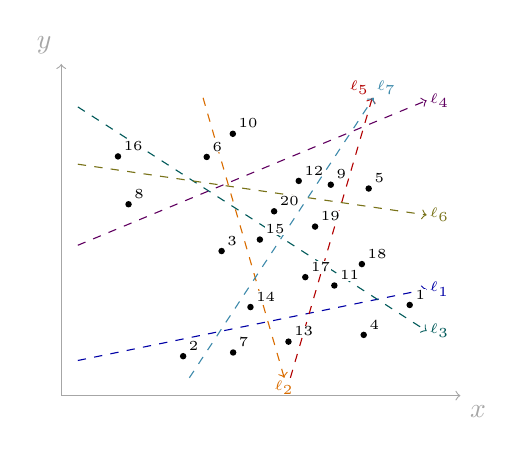
\begin{tikzpicture}[scale=0.78]
  \draw[->,gray!70] (0.45,0.45)--(6.95,0.45) node[below right] {$x$};
  \draw[->,gray!70] (0.45,0.45)--(0.45,5.85) node[above left] {$y$};
  \foreach \i/\linecolor/\xa/\ya/\xb/\yb/\labelanchor in {
    1/blue!65!black/0.72/1.022/6.4/2.182/west,
    2/orange!85!black/2.759/5.3/4.081/0.74/north,
    3/teal!70!black/0.72/5.151/6.4/1.502/west,
    4/violet!75!black/0.72/2.898/6.4/5.256/west,
    5/red!70!black/4.181/0.74/5.515/5.3/south east,
    6/olive!80!black/0.72/4.218/6.4/3.391/west,
    7/cyan!65!black/2.536/0.74/5.536/5.3/south west%
  } {
    \draw[->,color=\linecolor,dashed] (\xa,\ya)--(\xb,\yb);
    \node[anchor=\labelanchor,font=\tiny,text=\linecolor,inner sep=1pt]
      at (\xb,\yb) {$\ell_\i$};
  }
  \foreach \id/\x/\y in {
    1/6.124/1.926, 2/2.435/1.092, 3/3.061/2.804, 4/5.375/1.439,
    5/5.456/3.822, 6/2.819/4.336, 7/3.249/1.152, 8/1.546/3.566,
    9/4.839/3.884, 10/3.244/4.713, 11/4.897/2.243, 12/4.317/3.946,
    13/4.15/1.329, 14/3.531/1.892, 15/3.684/2.991, 16/1.374/4.345,
    17/4.424/2.379, 18/5.345/2.592, 19/4.583/3.202, 20/3.916/3.451
  } {
    \fill[black] (\x,\y) circle (1.5pt);
    \node[anchor=south west,font=\tiny,inner sep=0.4pt,fill=white,
          xshift=1.5pt,yshift=1.5pt] at (\x,\y) {\id};
  }
\end{tikzpicture}
\end{minipage}\hfill
\begin{minipage}[t]{0.60\textwidth}
\vspace{0pt}
\centering
{\small\textbf{One valid decision tree}\par}
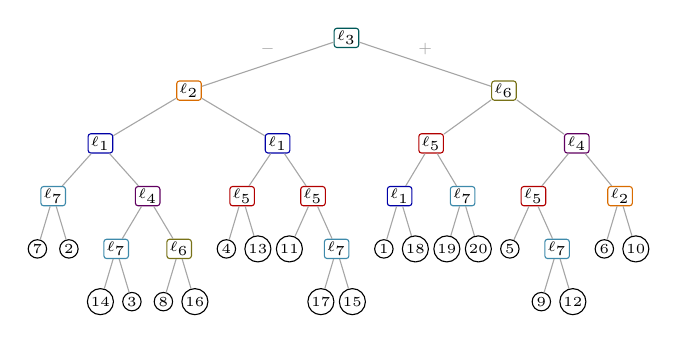
\begin{tikzpicture}[
  x=0.4cm,y=0.67cm,
  query/.style={rounded corners=1pt,fill=white,inner sep=1pt,font=\tiny},
  query1/.style={query,draw=blue!65!black},
  query2/.style={query,draw=orange!85!black},
  query3/.style={query,draw=teal!70!black},
  query4/.style={query,draw=violet!75!black},
  query5/.style={query,draw=red!70!black},
  query6/.style={query,draw=olive!80!black},
  query7/.style={query,draw=cyan!65!black},
  leaf/.style={draw,circle,fill=white,inner sep=0.7pt,font=\tiny},
  edge/.style={gray!70,thin}
]
  \node[query3] (n0) at (9.8125,0) {$\ell_3$};
  \node[query2] (n1) at (4.8125,-1) {$\ell_2$};
  \node[query1] (n2) at (2,-2) {$\ell_1$};
  \node[query7] (n3) at (0.5,-3) {$\ell_7$};
  \node[leaf] (n4) at (0,-4) {7};
  \node[leaf] (n5) at (1,-4) {2};
  \node[query4] (n6) at (3.5,-3) {$\ell_4$};
  \node[query7] (n7) at (2.5,-4) {$\ell_7$};
  \node[leaf] (n8) at (2,-5) {14};
  \node[leaf] (n9) at (3,-5) {3};
  \node[query6] (n10) at (4.5,-4) {$\ell_6$};
  \node[leaf] (n11) at (4,-5) {8};
  \node[leaf] (n12) at (5,-5) {16};
  \node[query1] (n13) at (7.625,-2) {$\ell_1$};
  \node[query5] (n14) at (6.5,-3) {$\ell_5$};
  \node[leaf] (n15) at (6,-4) {4};
  \node[leaf] (n16) at (7,-4) {13};
  \node[query5] (n17) at (8.75,-3) {$\ell_5$};
  \node[leaf] (n18) at (8,-4) {11};
  \node[query7] (n19) at (9.5,-4) {$\ell_7$};
  \node[leaf] (n20) at (9,-5) {17};
  \node[leaf] (n21) at (10,-5) {15};
  \node[query6] (n22) at (14.8125,-1) {$\ell_6$};
  \node[query5] (n23) at (12.5,-2) {$\ell_5$};
  \node[query1] (n24) at (11.5,-3) {$\ell_1$};
  \node[leaf] (n25) at (11,-4) {1};
  \node[leaf] (n26) at (12,-4) {18};
  \node[query7] (n27) at (13.5,-3) {$\ell_7$};
  \node[leaf] (n28) at (13,-4) {19};
  \node[leaf] (n29) at (14,-4) {20};
  \node[query4] (n30) at (17.125,-2) {$\ell_4$};
  \node[query5] (n31) at (15.75,-3) {$\ell_5$};
  \node[leaf] (n32) at (15,-4) {5};
  \node[query7] (n33) at (16.5,-4) {$\ell_7$};
  \node[leaf] (n34) at (16,-5) {9};
  \node[leaf] (n35) at (17,-5) {12};
  \node[query2] (n36) at (18.5,-3) {$\ell_2$};
  \node[leaf] (n37) at (18,-4) {6};
  \node[leaf] (n38) at (19,-4) {10};
  \foreach \parent/\child in {
    n3/n4, n3/n5, n7/n8, n7/n9, n10/n11, n10/n12,
    n6/n7, n6/n10, n2/n3, n2/n6, n14/n15, n14/n16,
    n19/n20, n19/n21, n17/n18, n17/n19, n13/n14, n13/n17,
    n1/n2, n1/n13, n24/n25, n24/n26, n27/n28, n27/n29,
    n23/n24, n23/n27, n33/n34, n33/n35, n31/n32, n31/n33,
    n36/n37, n36/n38, n30/n31, n30/n36, n22/n23, n22/n30%
  } {
    \draw[edge] (\parent)--(\child);
  }
  \draw[edge] (n0)--node[above,font=\tiny] {$-$} (n1);
  \draw[edge] (n0)--node[above,font=\tiny] {$+$} (n22);
\end{tikzpicture}
\end{minipage}
\caption{Seven randomly oriented supplied lines are drawn first, then
twenty hypotheses are placed in distinct cells of their arrangement.
The arrows orient the lines: the positive side is to the left of the
arrow. Each internal node queries the correspondingly colored line.
At every node the left branch is the negative answer and the right
branch is the positive answer. The leaf numbers match the point labels.
This valid tree has maximum depth five.}
\label{fig:problem-example}
\end{figure}

\subsection{Results and the main ideas}

We give polynomial-time constant-factor approximations for both
objectives:
\[
 4.464966
 \quad\text{for maximum depth},\qquad
 5.182976
 \quad\text{for expected depth}.
\]
The expected-depth bound applies to arbitrary strictly positive priors.
We first prove the individual-vertex factor below $5.445944$, then
improve it by applying the same polynomial coverage scheduler to
adjacent support blocks. Joint discovery and endpoint accounting
preserves the credit from a negative first endpoint. A coupled choice
of block orientations and geometric shift retains this saving through
the first two batches' coverage guarantees. Selectively querying both
endpoints after a positive answer also reveals pattern information;
a rational entropy lower bound credits it. Changing the initial
two coverage budgets and sometimes merging the first two geometric batches
gives the displayed expected-depth factor. A finite rational certificate
accounts for both delayed positive discoveries and the entire zero route.
For maximum depth, an exact rank-subset interval
scheduler with a logarithmic total cap, combined with the priority
fallback, lowers the polynomial factor from $5.464966$ to $4.464966$.
For every fixed $\varepsilon>0$, we give quasipolynomial-time
$(2+\varepsilon)$ approximations for both objectives, including
arbitrary-prior expected depth. A multigrade dynamic program schedules
adjacent hull-support blocks with nearly exact delay. Its direct
factors are below $4.464966$ for maximum depth and $3.7187$ for
expected depth; the former is also attained by the polynomial hybrid.
More significantly, the resulting bounds have leading
coefficient $2\lambda$ and an additive count or entropy potential.
Exact optimization of an initial $O(\log n)$ levels, followed by
these baseline trees, removes that potential from the final ratio.
The resulting running time is
$(mn)^{O(\varepsilon^{-1}\log n)}$ for $0<\varepsilon\le1$;
these guarantees are quasipolynomial.
Both exact threshold problems are strongly NP-complete. The
expected-depth reduction first uses strictly positive, polynomially
bounded integer weights before normalization. An exact geometric cloud
construction then gives strong NP-completeness under uniform priors.
The hardness instances
use integer-coordinate points on a parabola and only supplied line
queries. Constant-factor inapproximability remains open.

Two restricted algorithms sharpen this distinction. If a distinguished
hypothesis misses every designated cap and all caps have size at
most a fixed $b$, maximum depth is exactly solvable in polynomial
time. For weighted singleton/pair caps with all singleton tests and
a path-and-cycle pair graph, expected depth admits an EPTAS with
running time $2^{O(\varepsilon^{-3})}\operatorname{poly}(n,L)$.
The latter includes the weighted expected-depth hardness subclass:
an EPTAS is compatible with strong NP-completeness.
For uniform priors, a PTAS covers all fixed-size caps in convex
position with a distinguished all-miss hypothesis, even when singleton
tests are unavailable. Clearing short gaps separates bounded blocks;
an exact count-vector DP optimizes all interleavings of their queries.

The geometric structure behind the algorithms is easiest to see in a
state (the current set of hypotheses consistent with all answers so
far) where no line splits much of the remaining mass. Every test
then has a majority answer. The opposite, minority half-planes are
small, and Helly's theorem gives a point lying on all majority sides.
After translating this common witness to the origin, each query is
represented by a point in a normalized plane. The vertices of their
convex hull (the smallest convex set containing those points) suffice
to describe the relevant caps: each original cap is covered by at
most two adjacent vertex caps, and the vertex
answers of any one hypothesis form a \emph{circular interval}: a
consecutive block in the cyclic order in which the hull vertices
appear around the polygon, with wrap-around allowed. This turns the
geometric part of the problem into scheduling and searching over
circular intervals.

\paragraph{Maximum depth: schedule discovery against child heights.}
In a flat state, the algorithm first builds the recursive codes for
the hull-pattern classes. It then searches for a positive hull answer
using a schedule whose deadlines are derived from those codes' actual
heights. An optimal-tree path through the common witness supplies a
comparison schedule: classes that remain negative on a long prefix
have already saved that many queries when the optimal tree is
restricted to the class. Each original query has at most two
adjacent hull supports, so the comparison schedule consists of
singletons and adjacent pairs rather than arbitrary subsets.
Enumerating its first pair turns the remaining circular intervals
into ordinary intervals. A priority-greedy fallback preserves the
resulting credit simultaneously for every deadline. A second, exact
scheduler stores subsets of available ranks in a spatial Cartesian
tree. It is polynomial under a logarithmic total cap; simultaneous
recursive bounds for small and large optima make that cap sufficient
for the stronger general factor. Endpoint searches
are charged separately, with a smaller allowance when the discovery
path already supplies a negative neighbor. This is how the analysis
improves the constant without adding artificial height to a child
code.

\paragraph{Expected depth: pay once for learning a pattern.}
For expected depth, the algorithm again discovers the complete
hull-answer pattern before recursing. The analysis separates the
work into two parts. First, a class's constant prefix on an optimal
witness path disappears when the optimal tree is restricted to that
class; the saved queries pay for finding the class's first positive
hull answer. Second, the remaining endpoint information is paid for
by the entropy of the pattern that was not already revealed during
discovery. Exact weighted coverage at each integer budget, together
with a deterministic choice among shifted geometric batches, gives a
sharper first-cover bound. Adaptive block modes also credit the information
from a second endpoint answer, measured against a coarsened discovery
transcript whose cells retain the individual cap bound. A mass cap
on each adjacent support block
forces some targets into later blocks, where the discrete bound is
better; the waiting time of the all-zero pattern covers the
complementary case. Both the optimal-depth savings and the entropy
decrease telescope over the recursive partition, so no part of the
optimal cost is charged repeatedly.

\paragraph{Strong hardness: encode bin loads by matching choices.}
The reductions start from 3-Partition. Singleton and adjacent-pair
queries on disjoint odd paths make each item choose one of the
path's even-position vertices. A distinguished hypothesis forces
every optimal tree to make a maximum matching on these paths, so an
unmatched position represents a bin choice. For maximum depth,
clouds of points turn the resulting bin loads into counts of
branches with specified remaining heights. For expected depth,
carefully chosen weights turn them into a quadratic penalty for
unequal loads. The parabola construction realizes every query by an
explicit line. Replacing weight $w$ by a cloud of $w$ uniform points
with private singleton tests adds the same internal identification cost
to every matching invoice; this exact identity preserves the reduction.

Section~\ref{sec:preliminaries} fixes notation and provides the
coding, information, and geometry preliminaries.
Sections~\ref{sec:geometry} and~\ref{sec:worst} develop the
common-witness geometry and the maximum-depth algorithm.
Section~\ref{sec:mass-improvement}
establishes the initial expected-depth guarantee, and
Section~\ref{sec:polynomial-blocks} improves its polynomial factor.
Section~\ref{sec:adaptive-blocks} gives the sharper adaptive-mode
expected-depth algorithm, Section~\ref{sec:first-phase}
improves its initial batches, and Section~\ref{sec:polynomial-slots}
gives the polynomial maximum-depth improvement.
Section~\ref{sec:boundaries}
shows how to handle hypotheses on query lines, and
Section~\ref{sec:hardness} gives the reductions.
Section~\ref{sec:uniform-hardness} transfers hardness to uniform priors
through an exact geometric cloud identity. We first establish
the common-witness geometry and the accounting inequalities shared
by the algorithms; the later sections then apply them to the two
objectives separately. Section~\ref{sec:quasipolynomial} gives the
quasipolynomial improvements for both objectives using a spatial
multigrade dynamic program.
Section~\ref{sec:small-caps} gives the stronger small-cap algorithms.
